%This is my super simple Real Analysis Homework template

\documentclass{article}
\usepackage[utf8]{inputenc}
\usepackage[english]{babel}
\usepackage{amsmath,bm}
\usepackage{minted}
\usepackage[]{tcolorbox}
\usepackage[]{amsthm} %lets us use \begin{proof}
\usepackage[]{amssymb} %gives us the character \varnothing

\title{Homework 1}
\author{Guilherme Albertini}
\date\today
%This information doesn't actually show up on your document unless you use the maketitle command below

\begin{document}
\maketitle %This command prints the title based on information entered above

%Section and subsection automatically number unless you put the asterisk next to them.
\section*{Theory}
Let $Linear_1 \rightarrow f \rightarrow  Linear_2 \rightarrow g $ be a be a
two-layer neural net architecture whereby $Linear_i(x) =
  \bm{W}^{(i)}\bm{x}+\bm{b}^{(i)}$ is the $i^{th}$ affine transformation and
$f,
  g$ are element-wise nonlinear activation functions (else must use transposes and/or Hadamard products). When an input $\bm{x}\in
  \mathbb{R}^n$ is fed into the network, $\bm{\hat{y}} \in \mathbb{R}^K$ is
obtained as output.
%Basically, you type whatever text you want and use the $ sign to enter "math mode".
%For fancy calligraphy letters, use \mathcal{}
%Special characters are their own commands

\subsection*{Problem 1: Regression Task}
We would like to perform regression task. We choose
$f(\cdot)=5(\cdot)^{+}=5ReLU(\cdot)$ and $g$ to be the identity function. To
train, we choose MSE loss function,
$\ell_{MSE}(\bm{\hat{y}},\bm{y})=||(\bm{\hat{y}}-\bm{y})||^2$.
\begin{enumerate}
  \item Name and mathematically describe the 5 programming steps you
        would take to train this model with PyTorch using SGD on a single batch
        of data.
        \begin{tcolorbox}
          \begin{enumerate}
            \item First compute a prediction from the model (the forward pass); $\tilde{y}=model(x)$
            \item Second compute the loss through computation of the energy
            \item Zero the gradient parameters; $optimiser.zero\_grad()$
            \item Compute and accumulate gradient parameters; $L.backward()$
            \item Finally step in the opposite direction of the gradient; $optimiser.step()$
          \end{enumerate}
        \end{tcolorbox}
  \item For a single data point $(x,y)$, write down all inputs and outputs for
        forward pass of each layer. You can only use variables and mechanics specified
        prior in your answer.
        \begin{table}[]
          \begin{tcolorbox}
            \centering
            \begin{tabular}{|c|c|l|cc}
              \cline{1-3}
              \textbf{Layer}   & \textbf{Input} & \textbf{Output} &  &  \\ \cline{1-3}
              \textit{$Linear_1$} & $\bm{x}$              & $\bm{z_1}=\bm{W}^{(1)}\bm{x}+\bm{b}^{(1)}$               &  &  \\ \cline{1-3}
              \textit{f}       & $\bm{z_1}$              & $\bm{z_2}=5(\bm{W}^{(1)}\bm{x}+\bm{b}^{(1)})^+$               &  &  \\ \cline{1-3}
              \textit{$Linear_2$} & $\bm{z_2}$             & $\bm{z_3}=5\bm{W}^{(2)}(\bm{W}^{(1)}\bm{x}+\bm{b}^{(1)})^++\bm{b}^{(2)}$               &  &  \\ \cline{1-3}
              \textit{g}       & $\bm{z_3}$             & $\bm{z_3}$               &  &  \\ \cline{1-3}
              \textit{Loss}    & $\bm{z_3, y}$              & $||\bm{\hat{y}-y}||^2=||5\bm{W}^{(2)}(\bm{W}^{(1)}\bm{x}+\bm{b}^{(1)})^++\bm{b}^{(2)}-\bm{y}||^2$               &  &  \\ \cline{1-3}
              \end{tabular}
          \end{tcolorbox}
          \end{table}
          
  \item Write down the gradients calculated from the backward pass. You can only use the following variables: $\bm{x,y,W^{(1)},b^{(1)},W^{(2)},b^{(2)}}, \frac{\partial \ell}{\partial \bm{\hat{y}}}, \frac{\partial \bm{z_2}}{\partial \bm{z_1}},\frac{\partial \bm{\hat{y}}}{\partial \bm{z_3}}$, where $\bm{z_1,z_2,z_3,\hat{y}}$ are outputs of $Linear_1,f,Linear_2,g$, respectively.
        \begin{tcolorbox}
          \begin{flalign*}
            \frac{\partial \bm{z_{3i}}}{\partial \bm{W^{(2)}}}&=\frac{\partial (5\bm{W^{(2)}\max(0,W^{(1)}x+b^{(1)})+b^{(2)}})}{\partial \bm{W^{(2)}}}\\
            &=5\bm{\max(0,W^{(1)}x+b^{(1)})}^T \text{, else }0^T\\ 
            \frac{\partial \bm{z_{3}}}{\partial \bm{b^{(2)}}}&=\frac{\partial (5\bm{W^{(2)}\max(0,W^{(1)}x+b^{(1)})+b^{(2)}})}{\partial \bm{b^{(2)}}}\\
            &=diag(1)\\
            \frac{\partial \bm{\ell}}{\partial \bm{W^{(2)}}} &= \frac{\partial \bm{\ell}}{\partial \bm{\hat{y}}}\frac{\partial \bm{\hat{y}}}{\partial \bm{z_3}}\frac{\partial \bm{z_3}}{\partial \bm{W^{(2)}}} \\
            &=5\frac{\partial \bm{\ell}}{\partial \bm{\hat{y}}}\frac{\partial \bm{\hat{y}}}{\partial \bm{z_3}}\bm{\max(0,W^{(1)}x+b^{(1)})}^T\\
            \frac{\partial \bm{\ell}}{\partial \bm{b^{(2)}}} &= \frac{\partial \bm{\ell}}{\partial \bm{\hat{y}}}\frac{\partial \bm{\hat{y}}}{\partial \bm{z_3}}\frac{\partial \bm{z_3}}{\partial \bm{b^{(2)}}} \\
            &=\frac{\partial \bm{\ell}}{\partial \bm{\hat{y}}}\frac{\partial \bm{\hat{y}}}{\partial \bm{z_3}}\\
          \end{flalign*}
        \end{tcolorbox}
        \begin{tcolorbox}
          \begin{flalign*}
            \frac{\partial \bm{z_3}}{\partial \bm{z_2}}&=\frac{\partial (\bm{W^{(2)}}5\max(0,\bm{W^{(1)}x+b^{(1)}}))}{\partial 5 \max(0, \bm{W^{(1)}x+b^{(1)}})}=\bm{W^{(2)}}\\
            \frac{\partial \bm{z_{1i}}}{\partial \bm{W^{(1)}}}&= \frac{\partial (\bm{W^{(1)}x+b^{(1)}})}{\bm{W^{(1)}}}=x^T \text{, else }0^T\\
            \frac{\partial \bm{z_1}}{\partial \bm{b^{(1)}}}&= \frac{\partial (\bm{W^{(1)}x+b^{(1)}})}{\bm{b^{(1)}}}=diag(1)\\
           \frac{\partial \bm{\ell}}{\partial \bm{W^{(1)}}} &= \frac{\partial \bm{\ell}}{\partial \bm{\hat{y}}}\frac{\partial \bm{\hat{y}}}{\partial \bm{z_3}}\frac{\partial \bm{z_3}}{\partial \bm{z_2}}\frac{\partial \bm{z_2}}{\partial \bm{z_1}}\frac{\partial \bm{z_1}}{\partial \bm{W^{(1)}}} \\
            &= \frac{\partial \bm{\ell}}{\partial \bm{\hat{y}}}\frac{\partial \bm{\hat{y}}}{\partial \bm{z_3}}\bm{W^{(2)}}\frac{\partial \bm{z_2}}{\partial \bm{z_1}}\bm{x^T}\\
            \frac{\partial \bm{\ell}}{\partial \bm{b^{(1)}}} &= \frac{\partial \bm{\ell}}{\partial \bm{\hat{y}}}\frac{\partial \bm{\hat{y}}}{\partial \bm{z_3}}\frac{\partial \bm{z_3}}{\partial \bm{z_2}}\frac{\partial \bm{z_2}}{\partial \bm{z_1}}\frac{\partial \bm{z_1}}{\partial \bm{b^{(1)}}} \\
            &= \frac{\partial \bm{\ell}}{\partial \bm{\hat{y}}}\frac{\partial \bm{\hat{y}}}{\partial \bm{z_3}}\bm{W^{(2)}}\frac{\partial \bm{z_2}}{\partial \bm{z_1}}\\
          \end{flalign*}
        \end{tcolorbox}
  \item Show the elements of $\frac{\partial \bm{z_2}}{\partial \bm{z_1}}, \frac{\partial \bm{\hat{y}}}{\partial \bm{z_3}},\frac{\partial \ell}{\partial \bm{\hat{y}}}$. Be careful about dimensionality.
        \begin{tcolorbox}
          Note: $ i \in \left\lbrace1,\ldots,m\right\rbrace$ used throughout.
          \begin{flalign*}
            \frac{\partial \bm{z_2}}{\partial \bm{z_1}} &= \frac{\partial  (5\max(0,\bm{W^{(1)}x+b^{(1)}}))}{\partial (\bm{W^{(1)}x+b^{(1)}})}\\
            \left( \frac{\partial \bm{z_2}}{\partial \bm{z_1}}  \right)_{ii} &= \begin{cases} 0, & z_{1i} < 0 \\ 5, & z_{1i} > 0 \\ \text{undefined (or assigned a value 0 in code)}, & z_{1i} = 0 \end{cases}\\
            \text{Note: } \bm{z_1} &= \bm{W^{(1)}x+b^{(1)}}\text{ and the above is a diagonal matrix} \\
            \left(\frac{\partial \bm{\hat{y}}}{\partial \bm{z_3}}    \right)_{ii} &= 1 \text{ (and 0 elsewhere, off of diagonal; an identity matrix)}\\ 
            \frac{\partial \ell}{\partial \bm{\hat{y}}} &= \frac{\partial (||\bm{\hat{y}-y||^2})}{\partial \bm{\hat{y}}}=2\bm{{(\hat{y}-y)}^T} \text{ (A vector)}\\
          \end{flalign*}
        \end{tcolorbox}

\end{enumerate}

%If you want centered math on its own line, you can use a slash and square
%bracket.\\
%\[
%  \left \{
%  \sum\limits_{k=1}^\infty l(I_k):A\subseteq \bigcup_{k=1}^\infty \{I_k\}
%  \right \}
%\]
%The left and right commands make the brackets get as big as we need them to
%be.

\clearpage %Gives us a page break before the next section. Optional.
\subsection*{Problem 2: Classification Task}
We would like to perform multi-class classification task, so we set $f = tanh$ and $g = \sigma$, the logistic sigmoid function, $\sigma(z)=\frac{1}{1+\exp(-z)}$.
\begin{enumerate}
  \item If you want to train this network, what do you need to change in the equations of (1.2), (1.3) and (1.4), assuming we are using the same MSE loss function.
    \begin{tcolorbox}
      |$f$|\\ Input: $Linear_1(\bm{x})=\bm{W}^{(1)}\bm{x}+\bm{b}^{(1)}$\\
          Output ($z_2$): $f(Linear_1(\bm{x}))=\tanh(Linear_1(\bm{x}))\\
            =\tanh(\bm{W}^{(1)}\bm{x}+\bm{b}^{(1)})$\\
            $=\frac{\exp(\bm{W}^{(1)}\bm{x}+\bm{b}^{(1)})-\exp(-\bm{W}^{(1)}\bm{x}-\bm{b}^{(1)})}{\exp(\bm{W}^{(1)}\bm{x}+\bm{b}^{(1)})+\exp(-\bm{W}^{(1)}\bm{x}-\bm{b}^{(1)})}$\\
          |$Linear_2$|\\ Input: $f(Linear_1(\bm{x}))=\tanh(Linear_1(x))$\\
          Output ($z_3$): $Linear_2(f(Linear_1(\bm{x})))=\bm{W}^{(2)}\bm{f(Linear_1(\bm{x}))}+\bm{b}^{(2)}$\\
          $=\bm{W^{(2)}\tanh(W^{(1)}x+b^{(1)})+b^{(2)}}$\\
          |g|\\Input: $Linear_2(f(Linear_1(\bm{x})))$\\
          Output: $g(Linear_2(f(Linear_1(\bm{x})))) = \\
          \frac{1}{1+\exp(-z_3)}=\frac{1}{1+\exp(-(\bm{W^{(2)}\tanh(W^{(1)}x+b^{(1)})+b^{(2)}}))}=\bm{\hat{y}}$\\
          |Loss|\\
          Input: $\bm{\hat{y}}$\\
          Output: $||(\frac{1}{1+\exp(-(\bm{W^{(2)}\tanh(W^{(1)}x+b^{(1)})+b^{(2)}}))}-\bm{y})||^2$\\
    \end{tcolorbox}
    \begin{tcolorbox}
      \begin{flalign*}
        \frac{\partial \bm{z_{3i}}}{\partial \bm{W^{(2)}}}&=\frac{\partial (\bm{W^{(2)}\tanh(W^{(1)}x+b^{(1)})+b^{(2)}})}{\partial \bm{W^{(2)}}}\\
        &=\tanh(\bm{W^{(1)}x+b^{(1)}})^T \text{ , else }0^T\\
        \frac{\partial \bm{z_3}}{\partial \bm{b^{(2)}}}&=\frac{\partial (\bm{W^{(2)}\tanh(W^{(1)}x+b^{(1)})+b^{(2)}})}{\partial \bm{b^{(2)}}}\\
        &=diag(1)\\
        \frac{\partial \bm{\ell}}{\partial \bm{W^{(2)}}} &= \frac{\partial \bm{\ell}}{\partial \bm{\hat{y}}}\frac{\partial \bm{\hat{y}}}{\partial \bm{z_3}}\frac{\partial \bm{z_3}}{\partial \bm{W^{(2)}}} \\
        &=\frac{\partial \bm{\ell}}{\partial \bm{\hat{y}}}\frac{\partial \bm{\hat{y}}}{\partial \bm{z_3}}\tanh(\bm{W^{(1)}x+b^{(1)}})^T\\
        \frac{\partial \bm{\ell}}{\partial \bm{b^{(2)}}} &= \frac{\partial \bm{\ell}}{\partial \bm{\hat{y}}}\frac{\partial \bm{\hat{y}}}{\partial \bm{z_3}}\frac{\partial \bm{z_3}}{\partial \bm{b^{(2)}}} \\
        &=\frac{\partial \bm{\ell}}{\partial \bm{\hat{y}}}\frac{\partial \bm{\hat{y}}}{\partial \bm{z_3}}\\
      \end{flalign*}
    \end{tcolorbox}
    \begin{tcolorbox}
      \begin{flalign*}
        \frac{\partial \bm{z_3}}{\partial \bm{z_2}}&=\frac{\partial (\bm{W^{(2)}\tanh(W^{(1)}x+b^{(1)})+b^{(2)}})}{\partial \tanh(\bm{W^{(1)}x+b^{(1)}})}=\bm{W^{(2)}}\\
        \left(\frac{\partial \bm{z_2}}{\partial \bm{z_1}} \right)_{ii} &= \frac{\partial  (\tanh(\bm{W}^{(1)}\bm{x}+\bm{b}^{(1)}))}{\partial (\bm{W^{(1)}x+b^{(1)}})} = \bm{1}-{\tanh(\bm{W^{(1)}x+b^{(1)}})}^2\\
         \left( \frac{\partial \bm{\hat{y}}}{\partial z_3}   \right)_{ii} &= \frac{\partial ({1+\exp(-(\bm{W^{(2)}\tanh(W^{(1)}x+b^{(1)})+b^{(2)}}))})^{-1}}{\partial (\tanh(W^{(1)}x+b^{(1)})+b^{(2)})} \\
         &= \sigma(z_3)(1-\sigma(z_3))_i,\\ 
         &\text{ Note the two partials above represent diagonal matrices}  \\
         \frac{\partial \ell}{\partial \bm{\hat{y}}} &= \frac{\partial (||\bm{\hat{y}-y||^2})}{\partial \bm{\hat{y}}}=2\bm{{(\hat{y}-y)}^T} \text{ (A vector)}
      \end{flalign*}
    \end{tcolorbox}
  \item Now you think you can do a better job by using a Binary Cross Entropy (BCE) loss function $\ell_{BCE}(\bm{\hat{y},y})=\frac{1}{K}\sum_{i=1}^{K}-[y_i\log(\hat{y_i})+(1-y_i)\log(1-\hat{\hat{y_i}})]$. What needs to change from the previous?
      \begin{tcolorbox}
          |Loss|\\
          Input: $\bm{\hat{y}}$\\
          Output: $\ell_{BCE}(\bm{\hat{y},y})=\frac{1}{K}\sum_{i=1}^{K}-[y_i\log(\hat{y_i})+(1-y_i)\log(1-\hat{y_i})],$\\
          $\hat{y_i}=\frac{1}{1+\exp(-z_{3i})}$\\
          $\frac{\partial \ell}{\partial \hat{y}}=(\frac{-y}{\hat{y}}+\frac{1-y}{1-\hat{y}})^T\implies\frac{\hat{y_i}-y_i}{\hat{y_i}(1-\hat{y_i})}$
      \end{tcolorbox}
  \item Things are getting better. You realize that not all intermediate hidden activations need to be binary (or soft version of binary). You decide to use $f(\cdot)=(\cdot)^{+}$ but keep g as $\sigma$. Explain why this choice of f can be beneficial for training a (deeper) network.
      \begin{tcolorbox}
        Sigmoid function is more computationally intensive to compute compared to ReLU due to exponential operation; the latter produces sparsity in matrices which encourages numerical optimization techniques taking advantage of this time and space complexity reduction. 
      \end{tcolorbox}
      \begin{tcolorbox}
        ReLU also avoids the vanishing gradient problem, whereby the number of parameters receive very small updates such that the nodes deviate greatly from their optimal value. As the gradient is constant for ReLU compared to the sigmoid gradient always being smaller than 1, successive operations will start to prohibit learning.
      \end{tcolorbox}
\end{enumerate}

\subsection*{Problem 3: Conceptual Questions}
%
\begin{enumerate}
  \item Why is softmax actually softargmax?
    \begin{tcolorbox}
      The "softmax" is not a smooth approximation to the maximum function -- it is actually an approximation to the arg max function whose value is the index that has the maximum. Accordingly, some prefer the "softargmax" terminolgy to emphasize this distinction.
  \end{tcolorbox}
  \item Draw the computational graph defined by this function, with inputs $x, y, z \in \mathbb{R}$ and output $w \in \mathbb{R}$. You make use symbols $x, y, z,w$, and operators $+,\star$ in your solution. Be sure to use the correct shape for symbols and
  operators as shown in class.
  \begin{enumerate}
    \item $a = x \star y + z  $
    \item $b = (x+x) \star a$
    \item $w = a \star b$
  \end{enumerate}
  \includegraphics[width=15cm]{"diagram.jpg"}
  \item Draw the graph of the following:
    \begin{enumerate}
      \item ReLU()
      \begin{tcolorbox}
        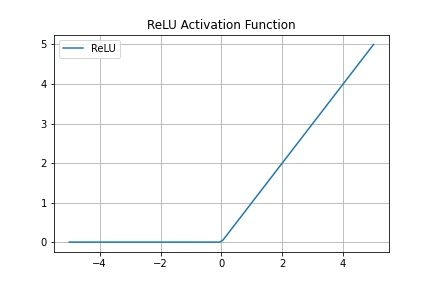
\includegraphics[width=9.5cm]{relu.jpg}
      \end{tcolorbox}
      \item LeakyReLU(neg slope is 0.01)
      \begin{tcolorbox}
        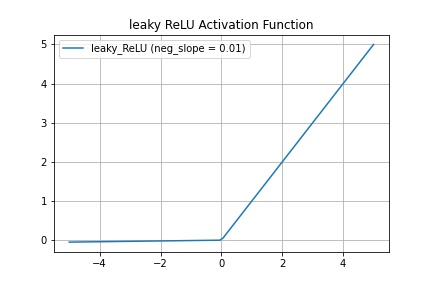
\includegraphics[width=9.5cm]{leaky_relu.jpg}
      \end{tcolorbox}
      \item Softplus(beta is 1)
      \begin{tcolorbox}
        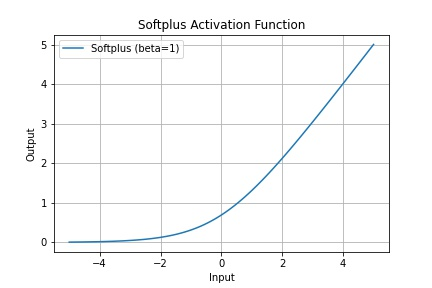
\includegraphics[width=9.5cm]{softplus.jpg}
      \end{tcolorbox}
      \item GELU
      \begin{tcolorbox}
        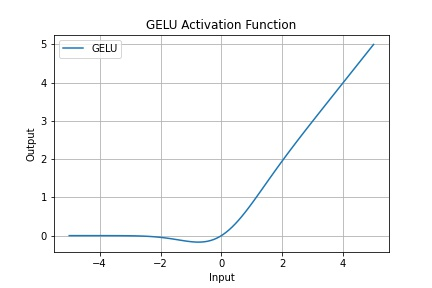
\includegraphics[width=9.5cm]{gelu.jpg}
      \end{tcolorbox}
    \end{enumerate} 
    \item What are 4 different types of linear transformations? What is the
    role of linear transformation and non linear transformation in a neural
    network?
    \begin{tcolorbox}
      Reflection, rotation, projection, and dilation are the main types of linear transformations. In neural networks, each output unit produces the linear combination of the inputs and the connection weights. Once we allow translation, these essentially become affine transformations. To introduce nonlinearity to the model, activation functions ingest these transformations through a nonlinear function and treat that as the unit output.
    \end{tcolorbox}
    \item Given a neural network F parameterized by parameters $\theta$, denoted $F_\theta$, dataset $D = x_1, x_2,\ldots, x_N $, and labels $Y = y_1, y_2,\ldots, y_N$, write down the mathematical definition of training a neural network with the MSE loss function $\ell_{MSE}(\bm{\hat{y},y})=||\hat{y}-y||^2$
    \begin{tcolorbox}
      \begin{flalign*}
        \theta_{i+1} = \theta_i - \alpha \frac{\partial \ell}{\partial \theta_i}
      \end{flalign*}
    \end{tcolorbox}
\end{enumerate}

\section*{Implementation}
%
\subsection*{Backpropagation }
You need to implement the forward pass and backward pass for Linear, ReLU, Sigmoid, MSE loss, and BCE loss in the attached mlp.py file. We provide three example test cases test1.py, test2.py, test3.py. We will test your implementation with other hidden test cases, so please create your own test cases to make sure your implementation is correct.
\subsection*{Gradient Descent}
Given a image classifier, implement a function that performs optimization on the input (the image), to find the image that most highly represents the class. Extra credit awarded for cool visuals. See gd.py.


\end{document}